\documentclass[9pt, twoside]{article}
\usepackage{multicol}
\usepackage{cite}
\usepackage{graphicx}
\usepackage{wrapfig}
\usepackage{float}
\usepackage{lipsum}
\usepackage{geometry}
\usepackage{hyperref}
\geometry{
a4paper,
tmargin=22mm,
rmargin=20mm,
lmargin=20mm,
}
\footskip=30pt

\begin{document}
\title {Model Predictive Control, Adaptive Control and System Identification - a Summary}

\author{Institut für Fluidsystmtechnik, Technische Universität Darmstadt}
\maketitle

\begin{abstract}
\end{abstract}

\begin{multicols}{2}
\section{Introduction}

\section{Materials and Methods}

\subsection{Model Predictive Control}

\subsection{Time Series Analysis}

\subsection{Time Series Forecasting}
\subsection{Adaptive Control}
This chapter provides an introduction to adaptive control and an overview of several important structures used in it. It offers a summary of the underlying principles and algorithms of each structure, while emphasizing on the characteristic differences between them. To shed some light on the practicality of adaptive control, some of the practical applications found in literature are also mentioned here.\\
\subsubsection{What is Adaptive Control?}
Intuitively, a characteristic property of adaptive controllers is their ability to adapt to changes in the dynamics of a process. Adaptive controllers gather information about an unknown process during operation and adjust their control laws in response to changes in the behaviour of the process. There are different ways of realizing adaptive control; however there is yet to be a formal definition distinguishing adaptive control from other control methods.\cite{aastrom2013adaptive} In principle, an adaptive controller must have adjustable parameters and a mechanism for adjusting those parameters. As shown in Figure \ref{Fig:General Structure}, the general structure of an adaptive control system can be viewed as having two closed loops; the inner loop  represents a typical feedback control loop consisting of the process and the controller, while the outer loop consists of the adjustment mechanism. \cite{Isermann:1992:ACS:573881} offers a classification of the different types of adaptive control shown in Figure REFERENCE.
\begin{figure}[H]
  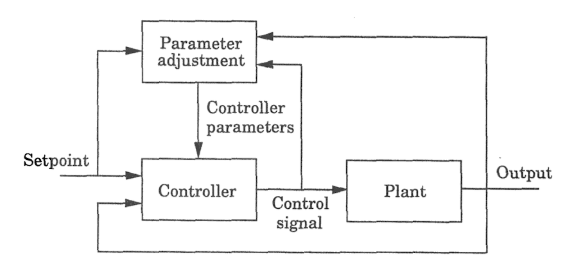
\includegraphics[width=0.9\linewidth]{General_Adaptive_Control.png}
  \caption{General Structure of an Adaptive Controller}
  \label{Fig:General Structure}
\end{figure}

\subsubsection{Feedforward vs. Feedback Adaptive Control}
Feedforward adaptive controllers require measurable signals that correlate well to the changing behaviour of the process. This type of adaptive controllers requires no feedback of the measured signals but rather an understanding of the process behaviour around operating conditions represented by those signals. Based on the operating conditions, the control law can then be adjusted to suit the changing properties of the process. One important example of feedforward adaptive control is gain scheduling, shown in Figure REFERENCE. For gain scheduling, different controller gains are usually designed a priori to be used in different operating conditions. Based on the measured signals, the operating condition is determined and the "scheduled" gains are used.\\
If the process behaviour cannot be directly determined by measuring process signals, a feedback adaptive controller must be used. Feedback adaptive controllers can be sub-categorized into dual and non-dual adaptive controllers. The objectives of dual adaptive controllers are twofold: optimizing a performance criterion to drive the output to the desired value, while minimizing the estimation error of the process parameters to improve the quality of future information. This approach is very complex and can only be solved numerically. It is, therefore, difficult to implement in practical application. \cite{aastrom2013adaptive} Non-dual adaptive controllers, however, only minimize a design performance criterion with no information about future estimates taken into account. The design of non-dual adaptive controllers is based on \textit{the separation principle}, which implies that the design of the estimation process is performed separately from the design of the controller. Moreover, non-dual adaptive controllers, with the exception of cautious controllers, use \textit{the certainty equivalence principle}. It is, therefore, assumed that the estimated process parameters are identical with the true parameters. \cite{Isermann:1992:ACS:573881} Two important types of non-dual adaptive controllers are Model Reference Adaptice Controllers (MRAC) and Mode Identification Adaptive Controllers (MIAC), which will be discussed in the following sections.
\subsubsection{Model Reference Adaptive Control (MRAC)}
Model Reference Adaptive Controllers were originally implemented in flight control using a model of the aircraft response to joystick motion.\cite{aastrom2013adaptive} They aim to achieve a closed loop performance close to that of the reference model by adjusting the controller parameters to minimize the difference $e=y-y_{m}$ between the output of the process and that of the reference model (Figure REFERENCE). There are various implementations of MRAC employing different adaptation laws. However, a common problem with MRACs is the fact that it only adapts if the input changes. Additionally, depending on the adaptation law, some MRACs are unstable under certain conditions. Moreover, the performance of MRACs is easily affected by noise and disturbances.
\subsubsection{Model Identification Adaptive Control (MIAC)}
Model Identification Adaptive Controllers are sometimes referred to as \textit{self-optimizing} or \textit{self-tuning controllers}. Unlike MRACs, this type of adaptive controllers does not aim to obtain the performance of one fixed reference model but rather estimates a model of the process at each step and adjusts the controller parameters accordingly. MIACs perform three tasks: estimate a model of the process based on its current behaviour, optimize the controller performance criterion and adjust the parameters of the controller. This control scheme is flexible in terms of the control algorithm and model estimation method. The model estimation can be implemented using various system identification methods described in (see \autoref{chap:SI}) or state estimation using observers or Kalman filters. Certainty equivalent controllers assume the estimated process model to be true, while cautious controllers take estimation errors into account and, in case of uncertainty, apply smaller values of the manipulated variable. Certainty equivalent controllers can be further subdivided into non-parametric and parametric adaptive controllers. The former use non-parametric identification methods such as time-response or frequency-response models, while the latter use parametric process models. The model estimation is performed only based on the inputs and outputs of the process, as shown in Figure REFERENCE.

\subsection{System Identification}
\label{chap:SI}
System Identification is the process of modelling the static and dynamic behaviour of a system and has a wide application area and an array of different implementation methods in engineering and economics. Choosing the right method is highly dependant on the application itself and requires some knowledge about the system. It is an iterative process that might require several trials before an adequate model is found.\newline
\\
 The three constituents of system identification are a data set, a set of candidate models and a set of criteria, based on which the most suitable model can be chosen. It is important to first set a clear purpose for this process. Decisions such as the desired type of model, the required accuracy, the available computing power and the intended use of the model are made during this phase. Then the suitable estimation method has to be determined based on the \textit{a priori} knowledge about the system and some engineering intuition. To select the appropriate estimation methods, one has to determine whether the system is \textit{linear} or \textit{non-linear}, \textit{time-variant} or \textit{-invariant} as well as other properties such as dead time and settling time. The amount of information available in this stage is crucial to the success of the whole process. Next, a measurement is planned to collect the required data. Here, one has to determine the input signals, sampling time and whether the measurement is to be performed on-line or offline. The data collected is then pre-processed and then a suitable identification method is applied. The resulting model is then validated by comparison of the plant output and model output to the same input. If the model does not pass the validation criteria, the whole process might have to be repeated.In the following sections, the most prominent estimation methods are summarized.\cite{isermann2010identification}\\
 \subsubsection{An Overview of Identification Methods}
\textit{Paramertic vs. Non-Parametric Methods}\\
\\
 The numerous methods available for system identification can be sorted into two main groups: \textit{non-parametric} and \textit{parametric methods}. Non-parametric methods do not explicitly search for a finite set of parameters to provide a mathematical model of the system. They rather search for a correlation between the inputs and outputs of the system either in the frequency domain or in the time domain. Among the non-parametric methods in the time domain are Transient-Response Analysis methods such as Impulse- or Step-Response Analysis, where a pulse or step signal is applied at the input and the output of the system is analysed to obtain the time-response coefficients. With frequency analysis, the aim is to determine the amplitude and phase shift of the output of the system to a sinusoidal input, for example. This process is then repeated for several frequency in the desired frequency band. With Fourier Analysis, it is even possible to apply multi-frequency inputs. There are several other correlation analysis methods that can be used in the time domain and the frequency domain. Non-parametric methods are practical in applications, where an explicit model of the system is needed. However, since the changing dynamics of the process in our application are also of interest, our focus lies on parametric system identification methods explained in the following sections.\\
 \\
 \textit{Models for Parametric Estimation}\\
 \\

 
 

\section{Computation}

\section{Model Validation}

\section{Discussion}


\section{Conclusion}


\section*{Acknowledgment}








\end{multicols}
\bibliography{quellen}{}
\bibliographystyle{plain}
\end{document}

